\documentclass{article}

\usepackage{neurips_2019_author_response}

\usepackage[utf8]{inputenc} % allow utf-8 input
\usepackage[T1]{fontenc}    % use 8-bit T1 fonts
\usepackage{hyperref}       % hyperlinks
\usepackage{url}            % simple URL typesetting
\usepackage{booktabs}       % professional-quality tables
\usepackage{amsfonts}       % blackboard math symbols
\usepackage{nicefrac}       % compact symbols for 1/2, etc.
\usepackage{microtype}      % microtypography
\usepackage{todonotes}
\usepackage{caption}

\begin{document}

%#3comparison of performance with the original models on a set of arithmetic tasks (significance: medium to low)

\paragraph{Why does the NALU perform great in the original paper?} %#3why does the multiplication perform satisfactory in the original paper, but fails in this paper. %#3 the paper does a superb analysis of the issues, but it is unclear whether these issues make the original model unusable (from the original paper it seems that is not the case) and how difficult do they make it train (what is the standard number of iterations NALU is trained for)?
We have contracted the authors of the original paper, unfortunately they have been unable to provide any specific details about the models or the experiments. As such, we firmly believe our implementation and experiments are identical to theirs. Our intuition about NALU is that convergence only happens for a luck initialization. In the original paper no analysis of ``success rate'' was done, and we thus believe their results are heavily cherry-picked. However, as we don't think such speculation is appropriate in a paper we have omitted that details. %#3how come NALU performs great in the original paper, but is often worse than the linear model in this paper? The difference wrt the results in the original paper needs to be properly explained in the paper. 
\textit{Why is the NALU worse than the linear model?} The NALU shares weights between the $\mathrm{NAC}_{+}$ and $\mathrm{NAC}_{\bullet}$ layers. Compared to a NALU with separated weights, we have observed that weight sharing makes addition harder but multiplication feasible when a gating mechanism is present. %#3the resulting experiments are specific to pick out the disadvantages of the original model 
\textit{Are the experiments designed to show a disadvantage with NALU?} No, our experiments are identical to those in the original paper. The parameters that we vary are those that are not stated in the original paper.

\vspace{-0.3cm} \paragraph{Is the comparison between NMU and $\mathrm{NAC}_{\bullet}$ unfair?} %#1It's not surprising to me that the proposed multiplication unit NMU outperforms $NAC_\cdot$, since $NAC_\cdot$ is targeting a more ambitious division operation as well, so the comparison is unfair. %#3Comparisons to the original model under the set of conditions of the original paper, and slowly showing/developing the issues of that model, i.e. starting with a fair comparison and then showing where the original model fails.\\
Maybe, it is true that our NMU model, unlike $\mathrm{NAC}_{\bullet}$, does not support division. On the other hand our model can understand inputs in the negative range. To make a more fair comparison, we have added two additional models. A variant called $\mathrm{NAC}_{\bullet, \sigma}$ that only supports multiplication, by constraining the weights with $W = \sigma(\hat{W})$ in $\mathrm{NAC}_{\bullet}$. And a variant of $\mathrm{NAC}_{\bullet, \sigma}$ that uses linear weights and bias regularization, identically to our NMU model, this model is called $\mathrm{NAC}_{\bullet, \mathrm{NMU}}$. Figure \ref{fig:sft-hidden-size} shows that both variations improve upon the original $\mathrm{NAC}_{\bullet}$ model, but not enough to be better than the NMU model. %#3Balance the conclusion, as it currently states the advantaged of NAU and NMU without mentioning their drawbacks, which seem significant wrt NALU.\\
\textit{The conclusion currently states the advantaged of NAU and NMU without mentioning their drawbacks.} Good point, we have fix that. Although, please note that the original paper also states that division does not extrapolate well. %#3Also, the presented models specialize for three arithmetic operations where the original model was tested on three more operations. #3Are these models applicable to those operations too?
\textit{$\mathrm{NAC}_{\bullet}$ supports $\sqrt{x}$ and $x^2$, does NMU support those?} Good point. NMU supports $x^2$, in the same way as $\mathrm{NAC}_{\bullet}$ does. It is just an easier version of multiplication. NMU does not support $\sqrt{x}$, we will mention that in the revision.

\vspace{-0.3cm}\begin{figure}[h]
\centering
\begin{minipage}{.48\textwidth}
  \centering
  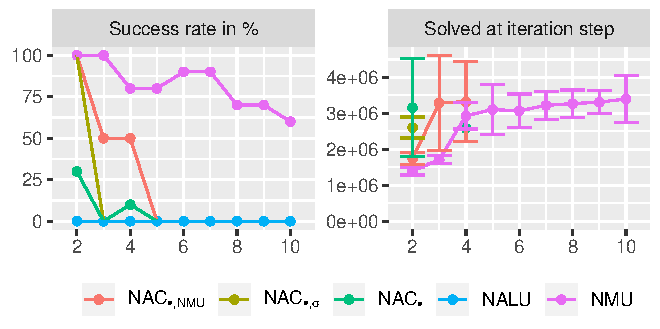
\includegraphics[width=\linewidth,trim={0 0 0 0},clip]{results-author-response/simple_function_static_mul_hidden_size.pdf}
  \vspace{-0.65cm}
  \captionof{figure}{Shows effect of increasing hidden size, thus adding redundant hidden units. Sparsity error excluded due to space constraints.}
  \label{fig:sft-hidden-size}
\end{minipage} \hspace{0.4cm}
\begin{minipage}{.48\textwidth}
  \centering
  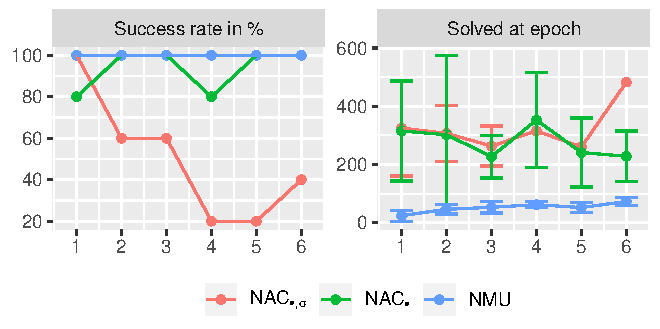
\includegraphics[width=\linewidth,trim={0 0 0 0},clip]{results-author-response/sequential_mnist_prod_hidden_size_small_l9.pdf}
  \vspace{-0.65cm}
  \captionof{figure}{Shows effect of the number of mnist hidden outputs, at sequence length 9, trained on sequence length 2. Sparsity error excluded due to space constraints.}
  \label{fig:test2}
\end{minipage}
\end{figure}

\vspace{-0.5cm} \paragraph{More experiments} We added experiments that tests the effect having redundant hidden units, this is important in applications where the correct number of hidden units is unknown. Additionally, we added the MNIST experiment from the original paper, although we test on multiplication instead of addition. This experiment evaluates how well a larger network can back-propagate though the $\mathrm{NAC}_{\bullet}$ or NMU layer. This experiment shows that the NMU allows for more than 10x faster learning. \textit{The novelty is only limited to the theoretical analyses of NALU and a new parameterization.} Our comparison should be on the baselines already established by the NALU paper, we thus don't want to invent new tasks. We hope that the additional experiments will convince you that our contributions are worth of publication.

% Put more emphasis on our ability to handle small and negative numbers.
\vspace{-0.3cm} \paragraph{If an initialization scheme results in $E[z_{h_l}] \ne 0$, does that mean the optimization would be necessarily difficult?} Not "necessarily", $E[z_{h_l}] = 0$ is a desirable not a theoretical necessarily. We use this desirable to inspire our model choice, and validate this choice in our experiments. Hopefully, our new comparison with $\mathrm{NAC}_{\bullet, \mathrm{NMU}}$ will convince you that this is a sensible desirable. We will make it more explicit that this is only a desirable in our revision. 

\vspace{-0.3cm} \paragraph{Other questions.} \textit{Would weight clipping have saturation issues?} No, because NMU is linear in $w_i$, the gradient is not affected by $w_i$. Gradients are derived in Appendix A. \textit{Does regularization in the NALU help?} $\mathrm{NAC}_{\bullet, \mathrm{NMU}}$ contains the regularization from NMU, but remains worse than NMU. There is no reason to believe that the added complexity of gating in NALU would make it better. \textit{Why did you chose $\lambda_{bias}$ in this way?} We found that learning interpolation and then sparsify to learn extrapolation are two different optimization problems. Only the latter, requires regularization. In our revision the bias regularizer is now scaled with spline function (shape similar to ReLU6). We explain this better in our revision. \textit{Is the parameter sparsity a necessity?} For multiplication it is a requirement. For addition and subtraction it helps with interpretability. \textit{Are the assumptions of splitting the NALU worth the effort?} NALU has its own issues, regarding the gating mechanism. However, we believe that before the gating issue can be solved the subunits needs to converge consistently. We hope future research will provide a solution to the gating mechanism issues present in NALU. \textit{Does the $\mathrm{NAC}_{+}$ need fixing?} Our NAU converges faster, uses half the parameters, and bias towards discrete weights. We believe these contributions are noteworthy, but agree that they are minor.

\vspace{-0.3cm} \paragraph{Minor typos and comments} Thanks for noticing, these issues have been fixed in our revision.

\end{document}